\section{Mathematical Framework (Conclusions and Future Work)}\label{sec:c10s2}
\kant[4-10]

This section builds on the material in \cref{sec:c10s1}, \cref{ch:1} and the prior work of \citet{main-2}; see also \citep{main-12,main-34}.

\begin{equation}\label{eq:c10s2-a}
  \hat{\theta} = \arg\min_{\theta\in\Theta}\; \frac{1}{n}\sum_{i=1}^{n}\ell\bigl(y_i, g_\theta(x_i)\bigr) + \lambda\lVert\theta\rVert_2^2 .
\end{equation}
Under standard regularity conditions the estimator is consistent, and its error satisfies
\begin{equation}\label{eq:c10s2-b}
  \mathbb{E}\lVert\hat\theta-\theta^\star\rVert^2 \le \frac{C\,\sigma^2 d}{n} + \lambda^2\lVert\theta^\star\rVert^2 .
\end{equation}

Equations~\eqref{eq:c10s2-a} and~\eqref{eq:c10s2-b} are used throughout the remainder of this section.

\kant[5-10]

\subsection{Quantitative behaviour}\label{sec:c10s2-q}
Results are collected in \cref{tab:c10s2} and visualised in \cref{fig:c10s2-f1}. Similar trends were reported in~\citep{main-21,main-36}.

\begin{table}[htbp]
\centering
\caption{Summary of measured quantities for experiment set \texttt{c10s2}.}\label{tab:c10s2}
\begin{tabular}{lrrr}
\toprule
Method & Score & Latency & Error \\
\midrule
Alpha & \num{52.6} & \SI{9.58}{\milli\second} & \num{1.286e-5} \\
Beta & \num{58.6} & \SI{9.89}{\milli\second} & \num{4.678e-1} \\
Gamma & \num{95.9} & \SI{4.86}{\milli\second} & \num{8.807e-5} \\
Delta & \num{72.6} & \SI{5.02}{\milli\second} & \num{5.653e-1} \\
Epsilon & \num{54.4} & \SI{2.63}{\milli\second} & \num{5.205e-2} \\
\bottomrule
\end{tabular}
\end{table}

\begin{figure}[htbp]
\centering
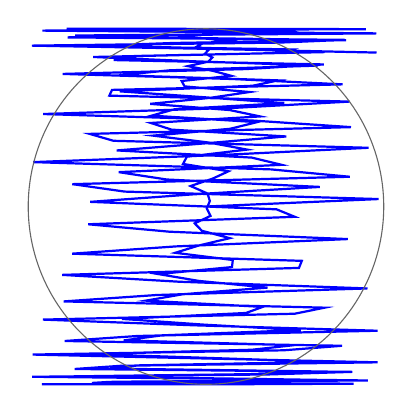
\begin{tikzpicture}\begin{axis}[width=0.7\linewidth,height=7cm,axis equal,hide axis]
\addplot[blue,thick,samples=200,domain=0:360]({sin(deg(3)*x/3)*cos(x)},{sin((4/3)*x*3/3)});
\addplot[black!60,samples=200,domain=0:360]({cos(x)*cos(deg(3*0))},{sin(x)});
\end{axis}\end{tikzpicture}
\caption{Generated figure for \texttt{c10s2-f1} (parameters $a=3$, $b=4$).}\label{fig:c10s2-f1}
\end{figure}

\lipsum[93-94]

\subsection{Implementation notes}\label{sec:c10s2-i}
The core routine is shown in \cref{lst:c10s2}; its complexity is $\mathcal{O}(N\log N)$ per iteration~\cite{main-35}.

\begin{lstlisting}[language=python,caption={Reference implementation for c10s2.},label={lst:c10s2}]
import numpy as np

def step(u, dt, dx, D):
    """Explicit finite-difference update."""
    lap = (np.roll(u, 1) - 2 * u + np.roll(u, -1)) / dx**2
    return u + dt * D * lap

u = np.exp(-((np.linspace(0, 1, 200) - 0.5) ** 2) / 0.01)
for _ in range(1000):
    u = step(u, 1e-5, 1 / 200, 1.0)
\end{lstlisting}

\kant[6-12]
\begin{theorem}\label{thm:c10s2}
Let $A\in\mathbb{R}^{n\times n}$ be symmetric positive definite with condition number $\kappa$. Then the iteration converges and
$\lVert e_k\rVert_A \le 2\bigl(\tfrac{\sqrt\kappa-1}{\sqrt\kappa+1}\bigr)^k\lVert e_0\rVert_A$.
\end{theorem}
\begin{enumerate}[label=(\roman*)]
\item the bound in \cref{thm:c10s2} is sharp for some initial errors;
\item the constant $2$ cannot be improved in general;
\item preconditioning reduces the effective $\kappa$.
\end{enumerate}

\begin{figure}[htbp]
\centering
\includegraphics[width=0.45\linewidth]{stripes.png}
\caption{Raster/vector asset \texttt{stripes.png} included from the figures directory.}\label{fig:c10s2-i0}
\end{figure}

\kant[2-12]
